\documentclass[12pt,german,a4paper]{article}

\usepackage[ngerman]{babel}
\usepackage{geometry} % alternatively type-area
\usepackage{fancyhdr}

% Font and Encoding Packages
% -----------------------------------------------------------------------
\usepackage[T1]{fontenc}    % enables symbols as ä, ö, ü, ß
\usepackage[utf8]{inputenc} % uft8-encoded symbols can processed
\usepackage{amsfonts}       % fonts mainly used in a mathematical context
\usepackage[lighttt]{lmodern}
%\usepackage[scaled=0.85]{DejaVuSansMono}

% Symbols
% -----------------------------------------------------------------------
% Specialized symbols
\usepackage{amssymb}	 % collection of mathematical symbols
\usepackage{extarrows}	 % collection of various arrows


% Maths Packages
% -----------------------------------------------------------------------
% These packages provide environments and commands for mathematical purposes
\usepackage{mathtools} % huge collection for mathematical writing replaces/extends amsmath
\usepackage{amsthm}    % provides claim-environments like theorem, lemma
\usepackage{cases}     % provides environment 'cases' for case distinctions
\usepackage{nicefrac}  % provides cmd 'nicefrac' to write '1/2' in texts


% Table and Picture Packages
% -----------------------------------------------------------------------
\usepackage{array}      % provides cmd to program talbes, e.g. with of a column
\usepackage{enumitem}   % user control over the basic list environments itemize, enumerate, and description
\usepackage{graphicx}   % provides optional arguments for 'includegraphics' like scaling
\usepackage{caption}    % enables description/captions for images, tables, algorithms
\usepackage{float}      % provides the 'H' option for floating objects like figures
\usepackage{pdfpages}   % enables the inclusion of PDFs in a latex document


% Computer Science Packages
% -----------------------------------------------------------------------
\usepackage[small]{complexity} % tool set for complexity theory
\usepackage{listings}          % integrate program source code into the pdf
\usepackage{algorithm}         % provides basic environment for algorithm display
\usepackage{algpseudocode}     % provides commands to write pseudocode
\usepackage{fancyvrb}


% Citation, Reference, Colours
% -----------------------------------------------------------------------
\usepackage{hyperref} % provides clickable in-document-references
\usepackage{xcolor}   % everything related to colours

\newcommand{\submissiontitle}[1]{
	\pagestyle{fancy}
	\setlength{\headheight}{14.5pt}
	\fancyhead[R]{\thepage}
	\fancyhead[L]{#1}
	\fancyfoot{}
	\title{#1}
}

%%%%%%%%%%%%%%%%%%%%%%%%%%%%%%%%%%%%%%%%%%%%%%%%%%%%%%%%%%%%%%%%%%%%%%%%%
% REDUCING the white part
%%%%%%%%%%%%%%%%%%%%%%%%%%%%%%%%%%%%%%%%%%%%%%%%%%%%%%%%%%%%%%%%%%%%%%%%%

\newgeometry{headheight=15.5pt, marginparwidth=2cm}
%\linenumbers

% allow page-breaks in mathematics mode but avoid them
\allowdisplaybreaks[1]


%%%%%%%%%%%%%%%%%%%%%%%%%%%%%%%%%%%%%%%%%%%%%%%%%%%%%%%%%%%%%%%%%%%%%%%%%
% Hyperlinks Setup
%%%%%%%%%%%%%%%%%%%%%%%%%%%%%%%%%%%%%%%%%%%%%%%%%%%%%%%%%%%%%%%%%%%%%%%%%

\hypersetup{
	colorlinks = true,		% instead of frames around the links, colour links
	linkcolor  = darkblue,  % colour internal links
	citecolor  = darkred,	% colour of citations
	urlcolor   = darkgreen	% colour of external links
}

%%%%%%%%%%%%%%%%%%%%%%%%%%%%%%%%%%%%%%%%%%%%%%%%%%%%%%%%%%%%%%%%%%%%%%%%%
% Colours
%%%%%%%%%%%%%%%%%%%%%%%%%%%%%%%%%%%%%%%%%%%%%%%%%%%%%%%%%%%%%%%%%%%%%%%%%

\definecolor{darkgreen}{rgb}{0,0.6,0}
\definecolor{darkred}{RGB}{185,40,25}
\definecolor{darkblue}{RGB}{0,95,140}
\definecolor{darkyellow}{RGB}{155,135,12}

\submissiontitle{Blatt 1 - Gruppe: G1-07}
\author{Mike Lenz, Jonas Tesfamariam} 

\begin{document}
\maketitle	
%--Content--

\section*{Aufgabe 1}
ID: 303ed1d1c1
\section*{Aufgabe 2}
\subsection*{a)}
Nein, es kann auch eine N:1 Beziehung sein. Ein Beispiel für solch eine Beziehung wäre ein Gebäude, welches mehrere Räume haben kann. Die Räume sind die schwache entity und das Gebäude die starke, wobei ein Gebäude mehrere Räume haben kann (Beispiel aus der Vorlesung: k02 Folie 28)
\subsection*{b)}
\begin{itemize}
\item Ein Tierarzt kann nur mit einem Medikament behandeln.
\item Es kann Tiere ohne Diagnose geben.
\item Mehrere Tiere können mit nur einem Medikament behandelt werden.
\item Bei jeder Diagnose kann nur ein Medikament verwendet werden.
\end{itemize}
\section*{Aufgabe 3}
\subsection*{a)}
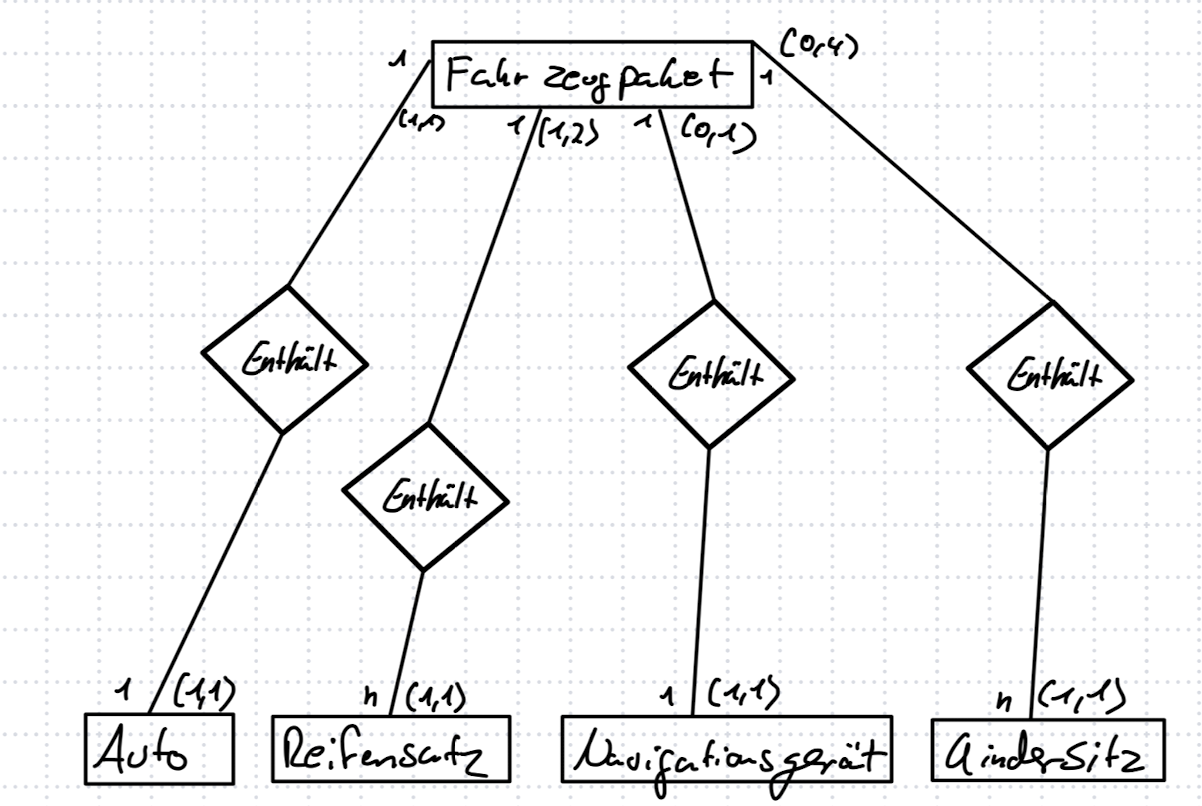
\includegraphics[width=\linewidth]{./img/aufgabe3a.png}
\subsection*{b)}
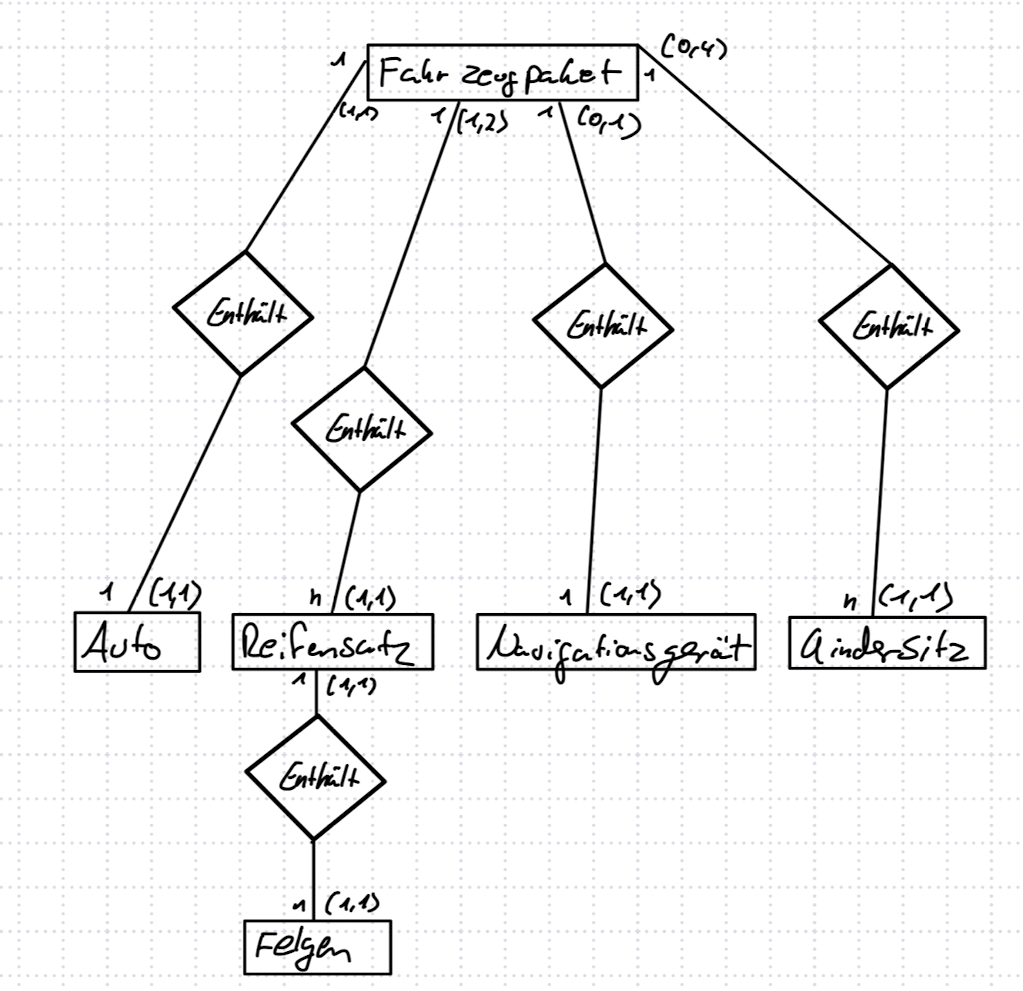
\includegraphics[width=\linewidth]{./img/aufgabe3b.png}
\section*{Aufgabe 4}
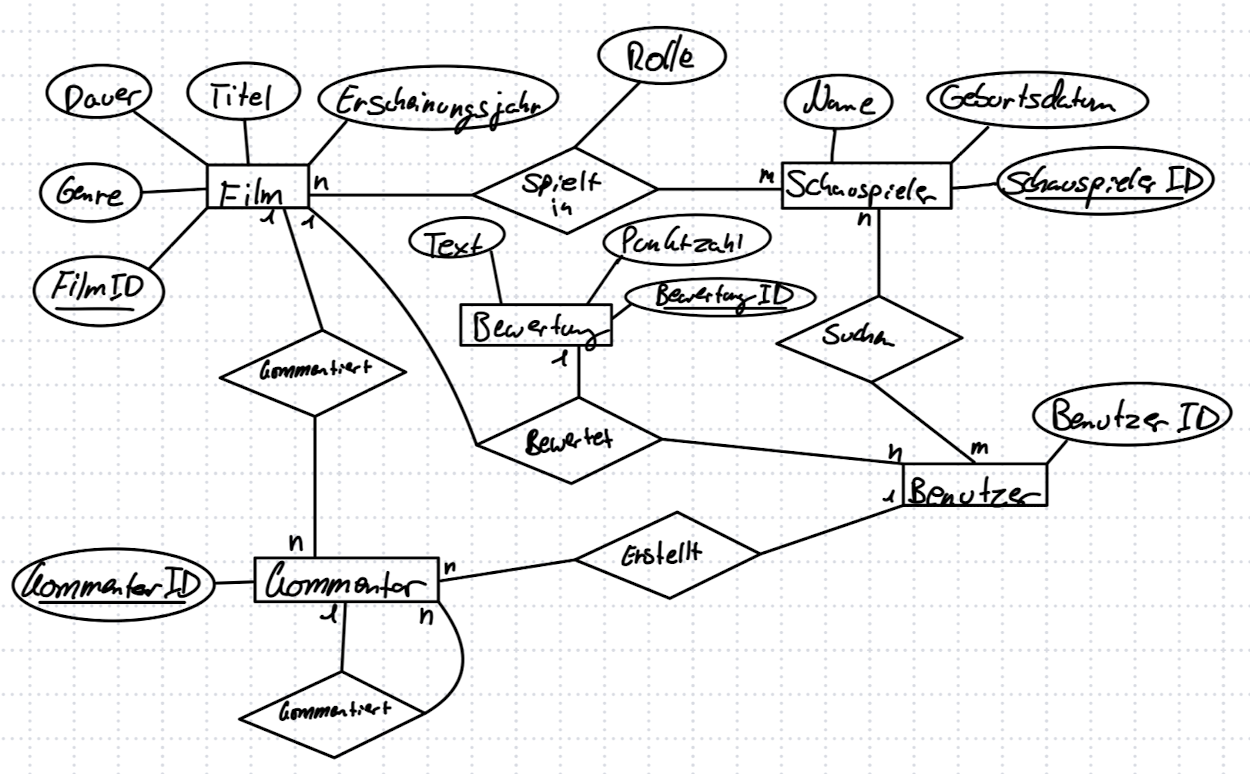
\includegraphics[width=\linewidth]{./img/aufgabe4.png}
Annahmen:
\begin{itemize}
\item Jede Entity erhält eine inkrementierende ID (Primarykeys sind für jede Entity benötigt).
\item Kommentare werden von Benutzern erstellt (Da sonst Niemand diese erstellt).
\end{itemize}
\end{document}